\chapter{Probas}

Neste capítulo detallaremos as probas realizadas para validar o noso sistema, tanto ao finalizar cada sprint coma ao rematar o desenvolvemento. Tamén se terán en conta aquelas ferramentas utilizadas para localizar e ter un maior control sobre os problemas da aplicación.

\section{Probas de validación de cada sprint}
Ao longo de todo o desenvolvemento do proxecto realizáronse probas ao finalizar cada sprint, ca fin de identificar posíbeis problemas introducidos sexa sobre as funcionalidades novas ou nas xa implementadas. A partir do terceiro sprint puidéronse realizar probas directamente sobre a aplicación pois nese momento xa se dispoñía dunha implementación básica que o permitía.

Estas probas realízanse utilizando a aplicación en condicións normais, tanto nun uso correcto coma nun uso erróneo para comprobar que non se producen situacións non controladas. Este uso erróneo consiste en intentar facer accións non permitidas, deixar sen cubrir certa información á hora de gardar datos, cambiar a pantalla rapidamente ou antes de que remate unha acción, etc...

As validacións destas probas realizáronse a dous niveis: a comprobación dun funcionamento correcto da aplicación a nivel de usuario e a revisión dos datos introducidos, modificados e eliminados da base de datos.

\begin{figure}[h]
	\begin{center}
		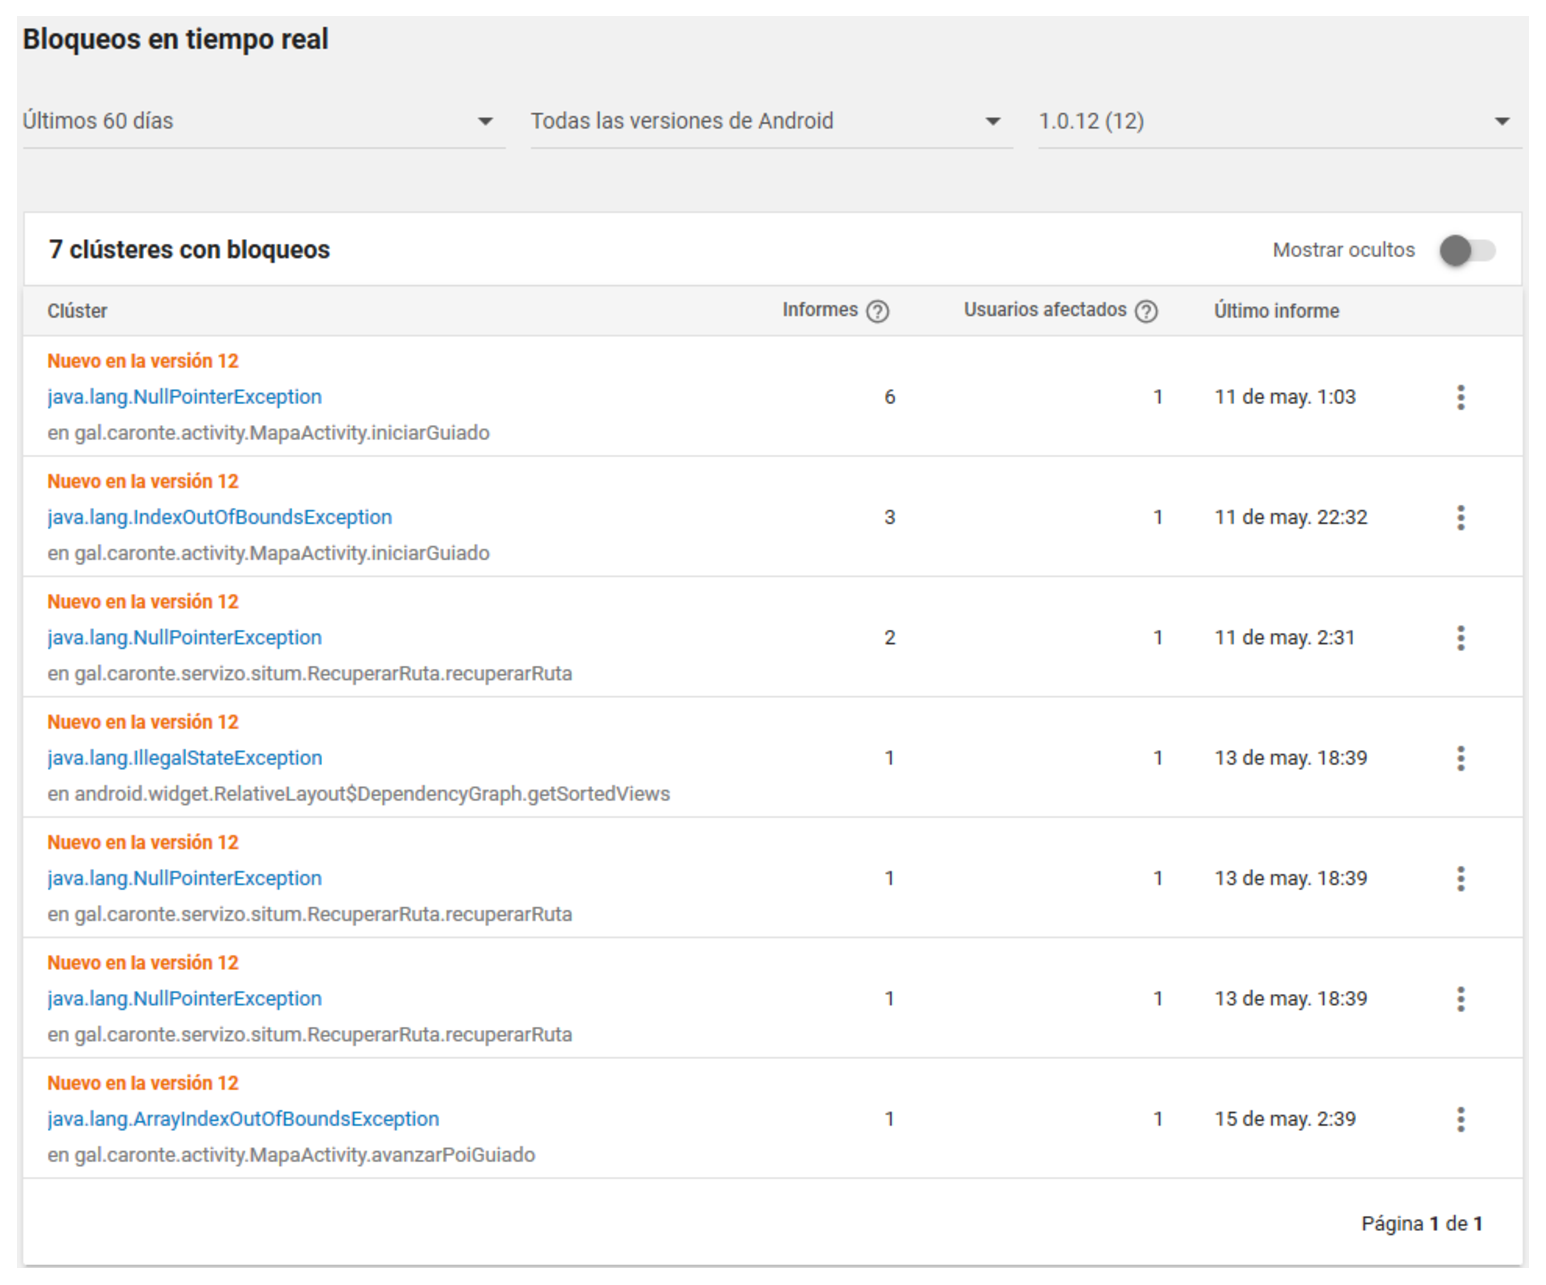
\includegraphics[width=1\textwidth]{figures/capturas/consolaGoogleBloqueos}
		\caption{Pantalla coas incidencias na consola de Google Play.}
		\label{fig:consolaGoogleBloqueos}
	\end{center}
\end{figure}

\section{Consola de Google}
Ao finalizar o terceiro sprint que xa supoñía unha aplicación usábel, aínda que limitada, procedeuse á publicación da aplicación en Google Play. Durante varios sprints foise publicando en modo Probas internas, sen permitir un acceso libre á mesma. Nesta modalidade permítese a proba dun número determinado de usuarios que se indican a través das súas contas de Google. Grazas a este sistema pódense recompilar os distintos erros que se produzan así como información sobre o dispositivo no que ocorren para poder dar unha solución con maior eficacia.
Despois do sexto sprint publicouse como beta aberta para poder acceder a un número maior de usuarios de proba. A publicación xera unha ligazón á aplicación que se pode compartir para que os usuarios a poidan descargar.

Dende a consola de Google tense acceso a información de todo tipo referente á aplicación, coma o número de descargas de cada versión publicada, o número de usuarios coa aplicación instalada, así como todos os envíos dos erros producidos nos terminais de proba (figura~\ref{fig:consolaGoogleBloqueos}), polo que resulta unha ferramenta moi útil para a depuración das incidencias atopadas polos usuarios que proban.


\section{Probas de rendemento}
As probas de rendemento realizáronse pensando no servidor do noso sistema e no servizo de Situm. Nun principio non se conta con que haxa problemas con ningún dos dous elementos, posto que o primeiro está despregado en Amazon Web Services e no caso de ter máis usuarios concurrentes do habitual disporíase do ancho de banda necesario; e o segundo xa está en uso en moitos puntos do planeta.

Para levar a cabo as probas, coordinouse o acceso ao sistema por parte de sete usuarios de proba para realizar todo tipo de accións dentro da aplicación, tanto de usuario normal coma de xestor de contido. Non se logrou un maior número de usuarios de proba por incompatibilidade horaria. En ningún momento se observou lentitude na aplicación e en todos os casos permitiu as accións sen amosar erros, incluso á hora de enviar e recibir imaxes o servidor.


\section{Enquisa usuarios}
Ao finalizar o desenvolvemento da sistema elaborouse unha breve enquisa para a valoración da aplicación Android entre os usuarios de proba. A idea da enquisa é que fosen preguntas breves e concisas, para que as persoas non dubidasen sobre a cuestión que se preguntaba. O sistema de puntuación é numérico, dende o 1 que indica o nivel máis baixo ata o 5 que indica o nivel máis alto.

As preguntas están divididas en catro bloques:
\begin{itemize}
	\item Usabilidade: cuestións sobre a facilidade de uso.
	\item Interface: preguntas sobre o atractiva que pode resultar visualmente e se está ben deseñada.
	\item Funcionalidade: cuestións sobre a utilidade da aplicación.
	\item Rendemento: preguntas sobre a velocidade e robustez.
\end{itemize}

\begin{table} [tbh]
	\footnotesize
	\centering
	\begin{tabular}{|l|c|}
		\hline 
		\textbf{Pregunta} & \textbf{Valoración media} \\ 
		\hline 
		\multicolumn{2}{ |c| }{USABILIDADE} \\ 
		\hline 
		É doada de usar? & 4,2 \\ 
		\hline 
		É intuitiva? & 3,4 \\ 
		\hline 
		Require pouco tempo de aprendizaxe? & 4,4 \\ 
		\hline 
		\multicolumn{2}{ |c| }{INTERFACE} \\ 
		\hline 
		O deseño é atractivo? & 2,8 \\ 
		\hline 
		As accións dispoñíbeis están claras? & 3,5 \\ 
		\hline 
		As accións dispoñíbeis están accesíbeis? & 4,3 \\ 
		\hline 
		\multicolumn{2}{ |c| }{FUNCIONALIDADE} \\ 
		\hline 
		É útil? & 4,4 \\ 
		\hline 
		Recomendaríaslla a outra persoa na mesma situación? & 4,4 \\ 
		\hline 
		As súas funcionalidades son únicas (non se atopan noutra aplicación)? & 4,1 \\ 
		\hline 
		\multicolumn{2}{ |c| }{RENDEMENTO} \\ 
		\hline 
		É estábel (sen erros)? & 4,4 \\ 
		\hline 
		É rápida nas súas accións? & 4,3 \\ 
		\hline 
	\end{tabular}
	\caption{Resultados da enquisa a usuarios.}
	\label{tab:enquisa}
\end{table}

Na táboa~\ref{tab:enquisa} poden observarse as preguntas realizadas aos usuarios de proba e a valoración media de cada unha delas. A enquisa foi respondida por 10 persoas, sendo a maioría delas xente á marxe do mundo do desenvolvemento de software.

Unha vez recollidas as valoracións e analizadas, pódese observar que o maior problema indicado polos usuarios da aplicación é que a súa interface non é agradábel. Coa intención de facer unha aplicación doada de usar e que requirise pouco tempo de aprendizaxe fíxose un deseño simple e funcional, mais de pouco atractivo visual, polo que en futuras modificacións habería que pensar en modificalo. Os outros dous puntos que requiren mellora sería o pouco intuitiva que resulta e que as accións dispoñíbeis non están o suficientemente claras.

Hai varios puntos fortes da aplicación, pero recalcaremos os de máis nota:
\begin{itemize}
	\item Require moi pouco tempo de aprendizaxe grazas á súa simpleza.
	\item A aplicación resulta útil para os usuarios.
	\item Recomendarían a outra persoa o uso da aplicación se se atopase nunha situación na que puidese ser usada.
	\item Non se localizaron erros na súa execución.
\end{itemize}